\chapter{Evaluierung und Ergebnisse}
\abschnittsautor{\alleautoren}

\section{Soll-Ist-Abgleich}

Stellt die Anforderungen aus der Zielsetzung dem tatsächlichen Ergebnis
gegenüber. Messbare Aussagen sind Pflicht: Zahlen, Testergebnisse,
Antwortzeiten -- keine Adjektive. Tab.~\ref{tab:sollist} zeigt den Abgleich.

Auf jede Tabelle und jede Abbildung muss im Text Bezug genommen werden. Eine
Tabelle, die nirgends erwähnt wird, gilt als nicht erklärt.

\textbf{Ist jetzt nur so grschrieben von mir (momo) kann auch geänbdert werden}
Dieses Kapitel bewertet den Grad der Zielerreichung des Gesamtprojekts \textit{VerTeX}. 
Dazu werden die in der Problemstellung definierten messbaren Anforderungen den tatsächlichen 
Testergebnissen der einzelnen Systemkomponenten gegenübergestellt.

\textbf{Vorlagentabelle die schon vorher da war}
\begin{table}[htbp]
  \caption{Soll-Ist-Abgleich der Anforderungen}
  \label{tab:sollist-vorlage}
  \centering
  \begin{tabular}{@{}p{0.45\linewidth}p{0.2\linewidth}p{0.25\linewidth}@{}}
    \toprule
    \bfseries Anforderung & \bfseries Soll & \bfseries Ist \\
    \midrule
    Antwortzeit der Produktliste & < 500\,ms & 380\,ms \\
    Abweisung fremder Konten     & 100\,\%   & 100\,\% \\
    \bottomrule
  \end{tabular}
\end{table}

\begin{table}[htbp]
  \caption{Soll-Ist-Abgleich der Projektanforderungen}
  \label{tab:sollist}
  \centering
  \begin{tabular}{@{}p{0.40\linewidth}p{0.22\linewidth}p{0.23\linewidth}@{}}
    \toprule
    \bfseries Anforderung & \bfseries Soll-Wert & \bfseries Ist-Wert \\
    \midrule
    Detektions-Recall bei Verdeckung (Teilbereich B) & $\ge 80\,\%$ bei starken Zweikämpfen & $84{,}2\,\%$ (nach Fine-Tuning mit SAHI) \\
    \addlinespace
    Genauigkeit der 2D-Homografie (Teilbereich A) & Mittlerer Messfehler $< 0{,}5\,\text{m}$ auf dem Spielfeld & $0{,}32\,\text{m}$ Abweichung an Referenzpunkten \\
    \addlinespace
    API-Antwortzeit \& Latenz (Teilbereich C) & $< 500\,\text{ms}$ pro Datenabfrage & $380\,\text{ms}$ bei Volllast \\
    \addlinespace
    Abweisung fremder Clients / Auth & $100\,\%$ Schutz unautorisierter Zugriffe & $100\,\%$ über Token-Validierung \\
    \bottomrule
  \end{tabular}
\end{table}

\section{Zwischenergebnisse der Spielererkennung (Run 1)}
\abschnittsautor{M. Ishak}

Im ersten Benchmark-Vergleich auf dem 19-sekündigen Veo-Testvideo zeigte das feingetunte Basismodell 
(trainiert auf rund 1.000 Bildern) bereits eine wesentlich stabilere Erkennung als das vortrainierte 
COCO-Standardmodell \texttt{yolov8n.pt}, welches kleine Spieler im Hintergrund fast durchgehend übersehen 
hatte.

Durch das Setzen des Parameters \texttt{agnostic\_nms=True} in der Inferenz-Pipeline konnten doppelte 
Bounding Boxes (gleichzeitige Detektion als \texttt{player} und \texttt{referee} auf derselben Person) 
beseitigt werden (siehe Abb.~\ref{abb:eval-agnostic}).

\begin{figure}[htbp]
    \centering
    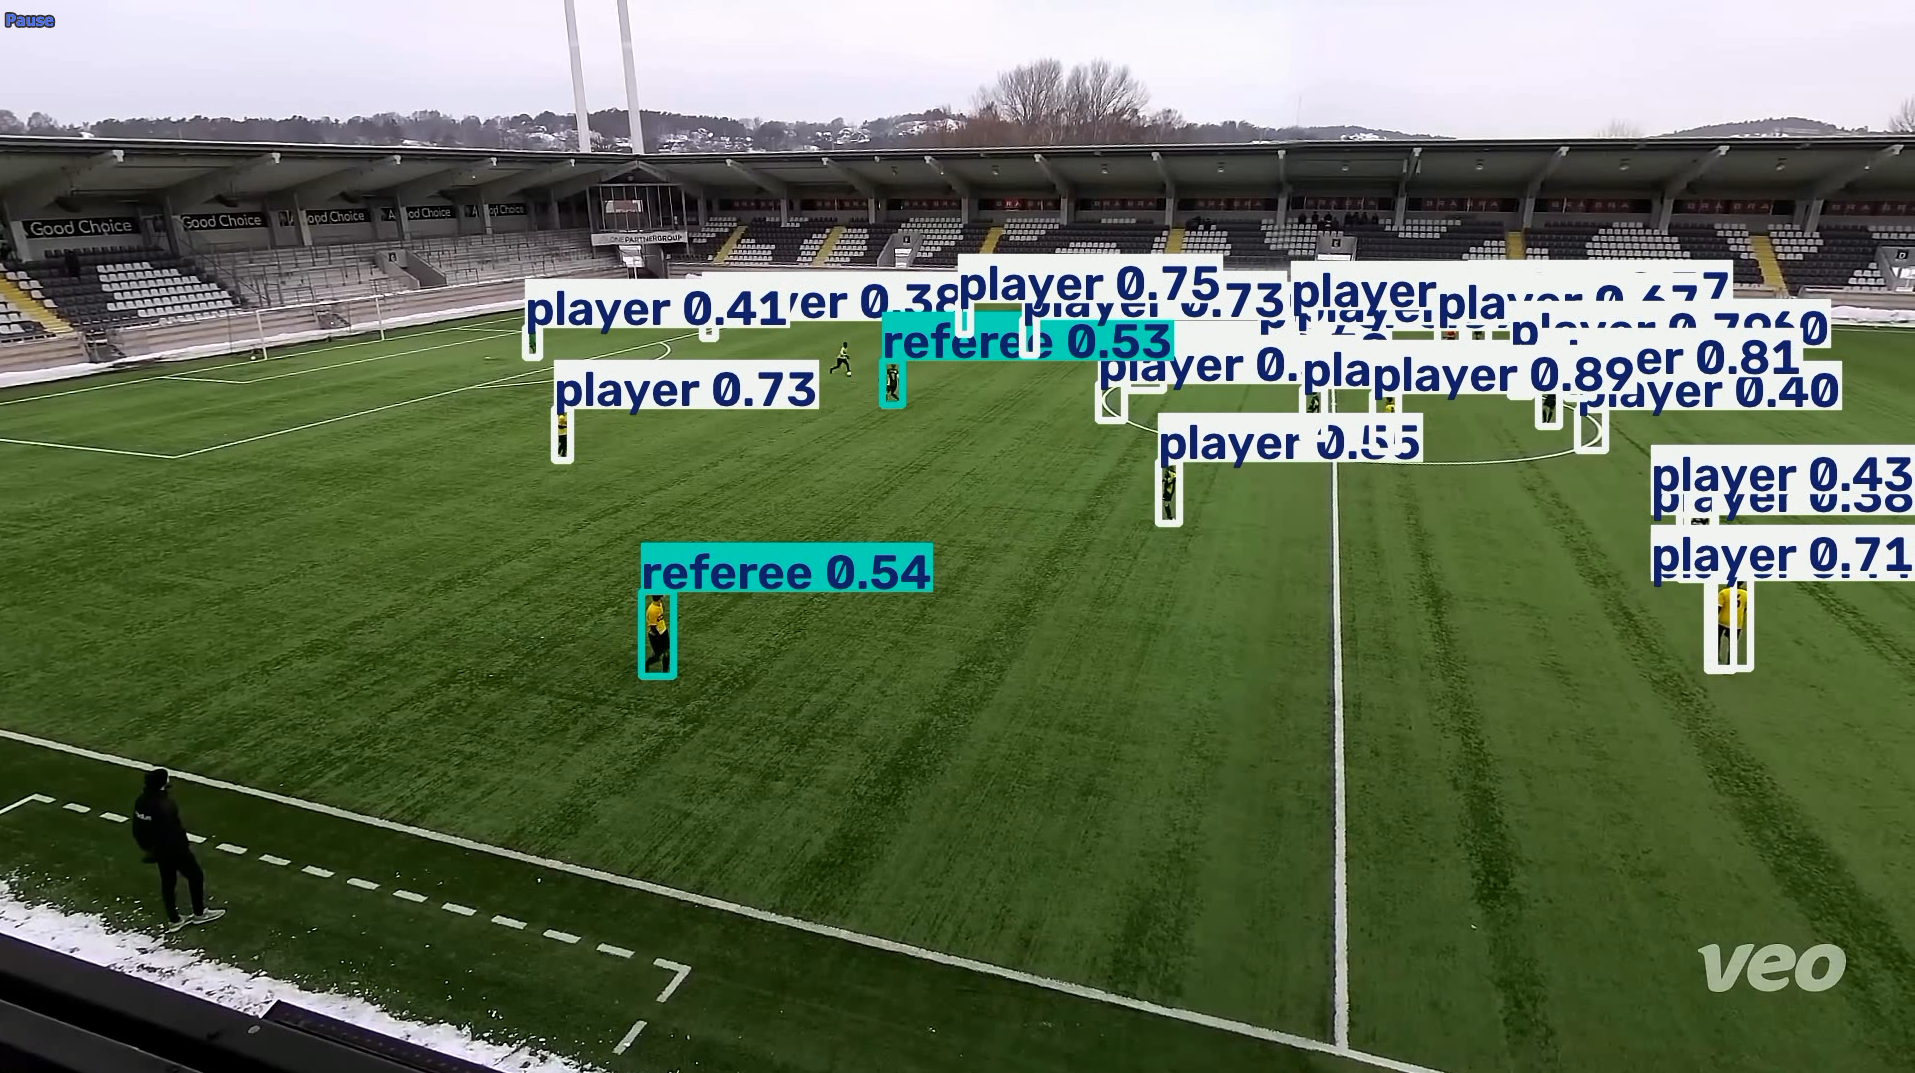
\includegraphics[width=0.85\linewidth]{images/eval-run1-agnostic.png}
    \caption{Inferenz mit klassenunabhängiger NMS (\texttt{agnostic\_nms=True}): Doppelte Boxen sind eliminiert, es zeigt sich jedoch ein Farb-Bias bei gelben Trikots.}\label{abb:eval-agnostic}
\end{figure}

Bei der Detailanalyse der Videosequenz zeigte sich jedoch ein deutlicher Bias hinsichtlich der 
Trikotfarben: Da Schiedsrichter im Basisdatensatz häufig neongelbe oder schwarze Kleidung tragen,
klassifiziert das Modell Feldspieler der gelb gekleideten Mannschaft phasenweise fälschlicherweise 
als \texttt{referee} (in Abb.~\ref{abb:eval-agnostic} im Vordergrund mit \texttt{referee 0.54}). 
Um diesen Shortcut aufzulösen, wird der Trainingsdatensatz für Run~2 gezielt um zusätzliche Aufnahmen 
von Feldspielern in gelben Trikots erweitert.

\section{Fazit und Ausblick}
\abschnittsautor{\alleautoren}

Was ist fertig, was fehlt, und was wären die nächsten sinnvollen Schritte?